\section{Benchmark Results}
\label{cha:results}

In this section, we present and compare the findings from the data analysis across each targeted datastore. Throughout the benchmarking sessions, no CPU performance issues were detected on the client side (workload generator), ensuring that client limitations did not impact latency measurements. Additionally, the error rate consistently remained zero for all runs, indicating that every read request was completed.

\paragraph*{EC2-RDS vs. Lambda-RDS}
EC2-RDS outperforms Lambda-RDS by approximately $51\%$ under constant load and $56\%$ under burst workload. Furthermore, EC2-RDS exhibits $41\%$ and $45\%$ less standard deviation than Lambda-RDS under constant and burst workload, respectively. As shown in \hyperref[fig]{Figure 4.2.1}, the latency for Lambda-RDS often experiences abrupt increases or decreases, persisting at such levels for several hours. This behavior makes Lambda-RDS less stable and predictable compared to EC2-RDS. A possible cause is that the underlying cloud infrastructure conditions fluctuate, leading to inconsistent latency performance \cite{}.

\paragraph*{EC2-DynamoDB vs. Lambda-DynamoDB} EC2-DynamoDB outperforms Lambda-DynamoDB by approximately $14\%$ under constant load and $16\%$ under burst workload. Furthermore, Lambda-DynamoDB exhibits $20\%$ and $7\%$ less standard deviation than EC2-DynamoDB under constant and burst workload, respectively.

\paragraph*{EC2-S3 vs. Lambda-S3}
EC2-S3 outperforms Lambda-S3 by approximately $8\%$ under constant load and $10\%$ under burst workload. Additionally, Lambda-S3 exhibits $22\%$ less standard deviation than EC2-S3 under constant load but $12\%$ more under burst workload. As illustrated in \hyperref[fig:bar_s3_const]{Figure 4.1.5}, the variance of EC2-S3 under constant load is approximately three times higher than under burst workload, as shown in \hyperref[fig:bar_s3_bursty]{Figure 4.1.6}. This observation appears counterintuitive. Due to the constraints of AWS Free Tier, experiments involving S3 were shorter, as discussed in \cref{cha:implementation}, which may have amplified the impact of fluctuations in the underlying cloud infrastructure \cite{}.

We observe that EC2 pairs consistently outperform Lambda pairs across all experiments. However, the absolute difference in mean latencies remains below 1.34 milliseconds. We know that Lambda functions run within Firecracker VMs, which are deployed on multi-tenant EC2 instances. Communication between Lambda functions and their host EC2 instances occurs via a virtio-based interface, introducing additional networking overhead of approximately $0.06ms$ \cite{}. However, this overhead appears negligible compared to the observed differences, suggesting that additional factors contribute to the latency variations.

\paragraph*{Outliers}
--> TODO <--

\begin{figure}[h]
	\caption{--> TODO: Add latency CDF graphs here <--}
\end{figure}

\begin{figure}[h]
	\begin{subfigure}{0.49\linewidth}
		\centering
		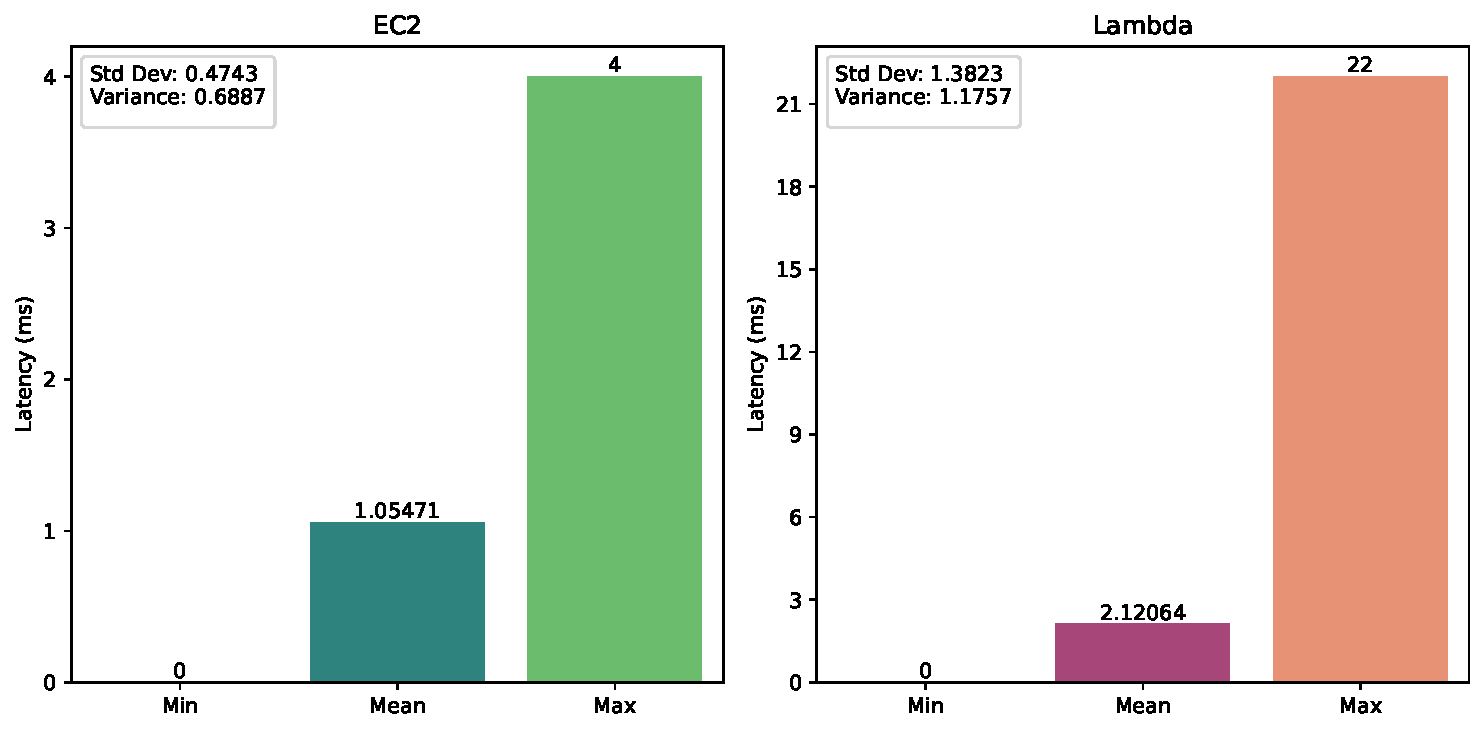
\includegraphics[width=\linewidth]{./fig/bar-rds-constant.pdf}
		\caption{Constant Workload on RDS}
		\label{fig:bar_rds_const}
	\end{subfigure}
	\hfill
	\begin{subfigure}{0.49\linewidth}
		\centering
		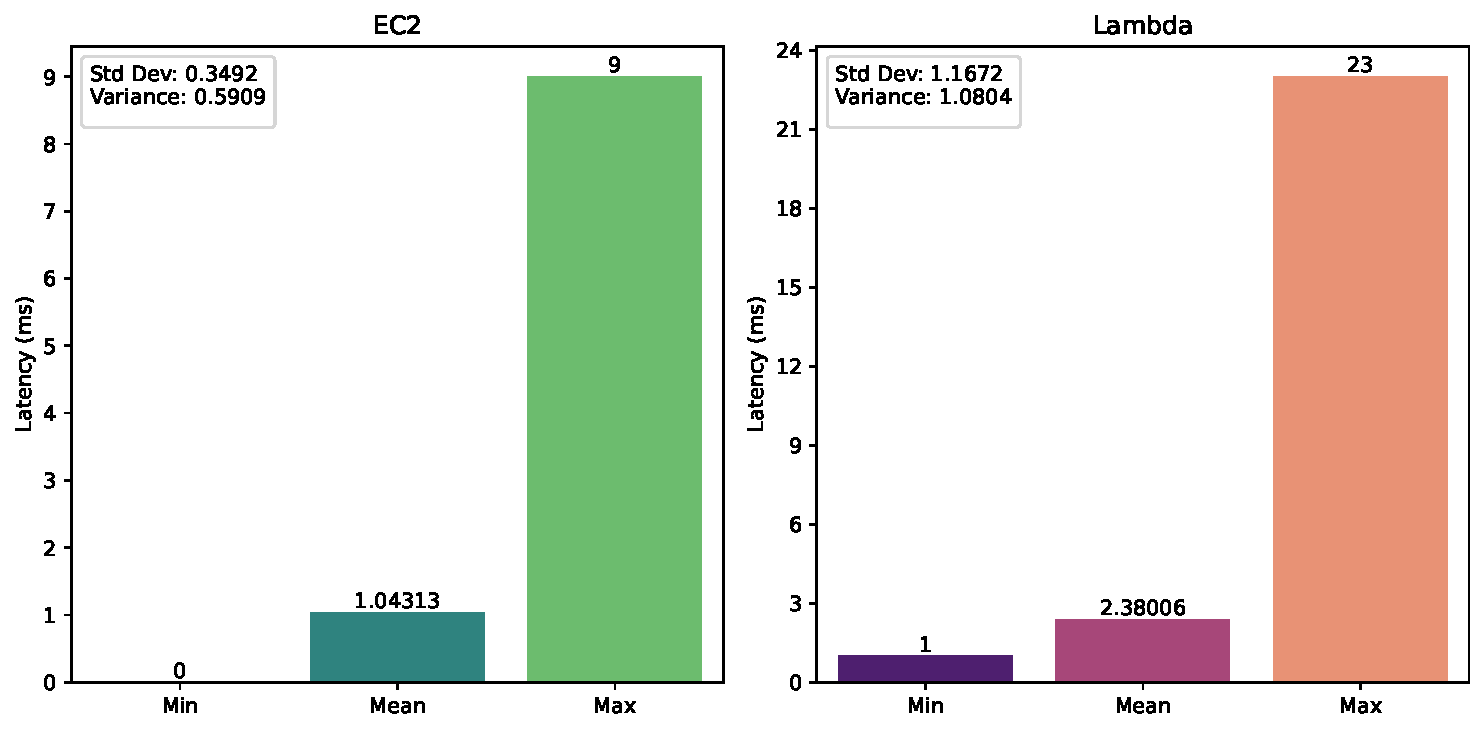
\includegraphics[width=\linewidth]{./fig/bar-rds-bursty.pdf}
		\caption{Burst Workload on RDS}
		\label{fig:bar_rds_bursty}
	\end{subfigure}
	\vfill
	\begin{subfigure}{0.49\linewidth}
		\centering
		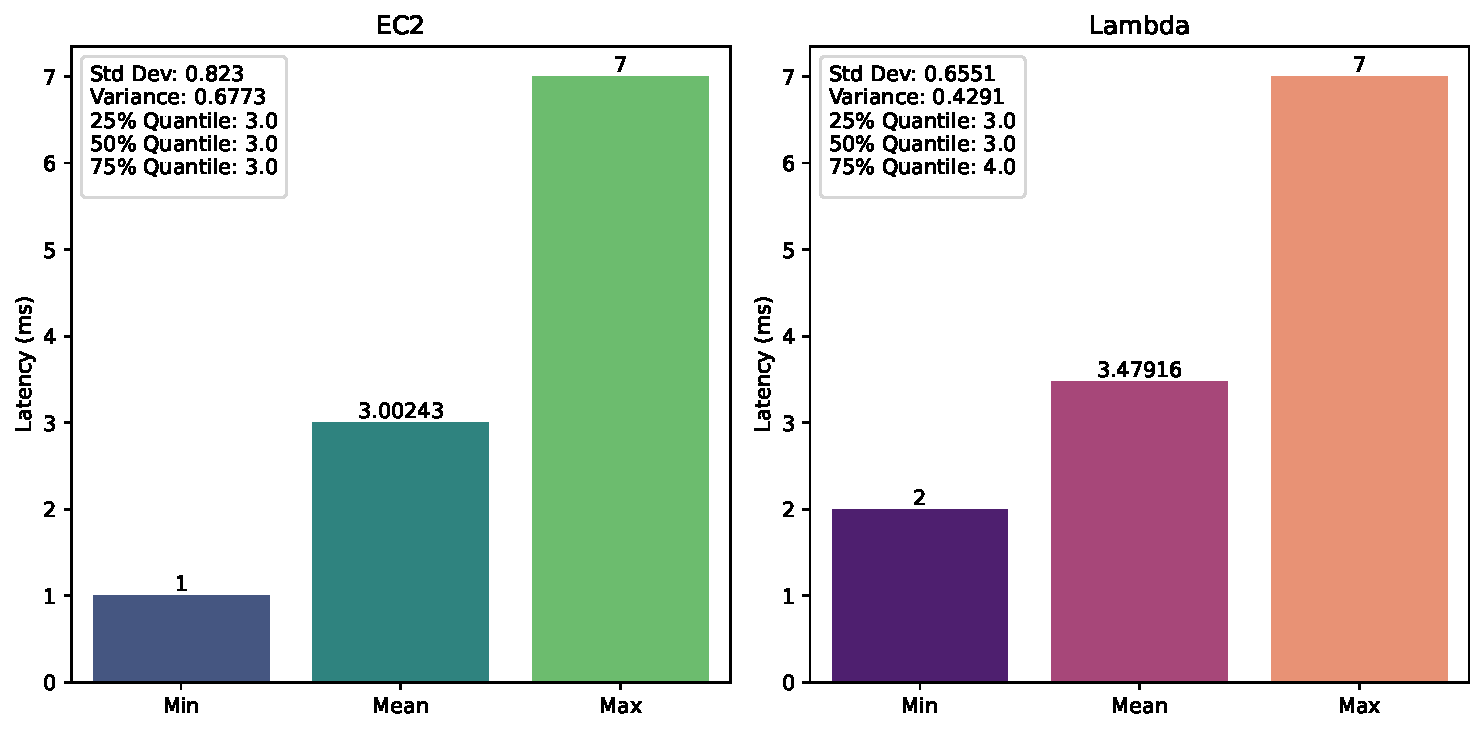
\includegraphics[width=\linewidth]{./fig/bar-dynamo-constant.pdf}
		\caption{Constant Workload on DynamoDB}
		\label{fig:bar_ddb_const}
	\end{subfigure}
	\hfill
	\begin{subfigure}{0.49\linewidth}
		\centering
		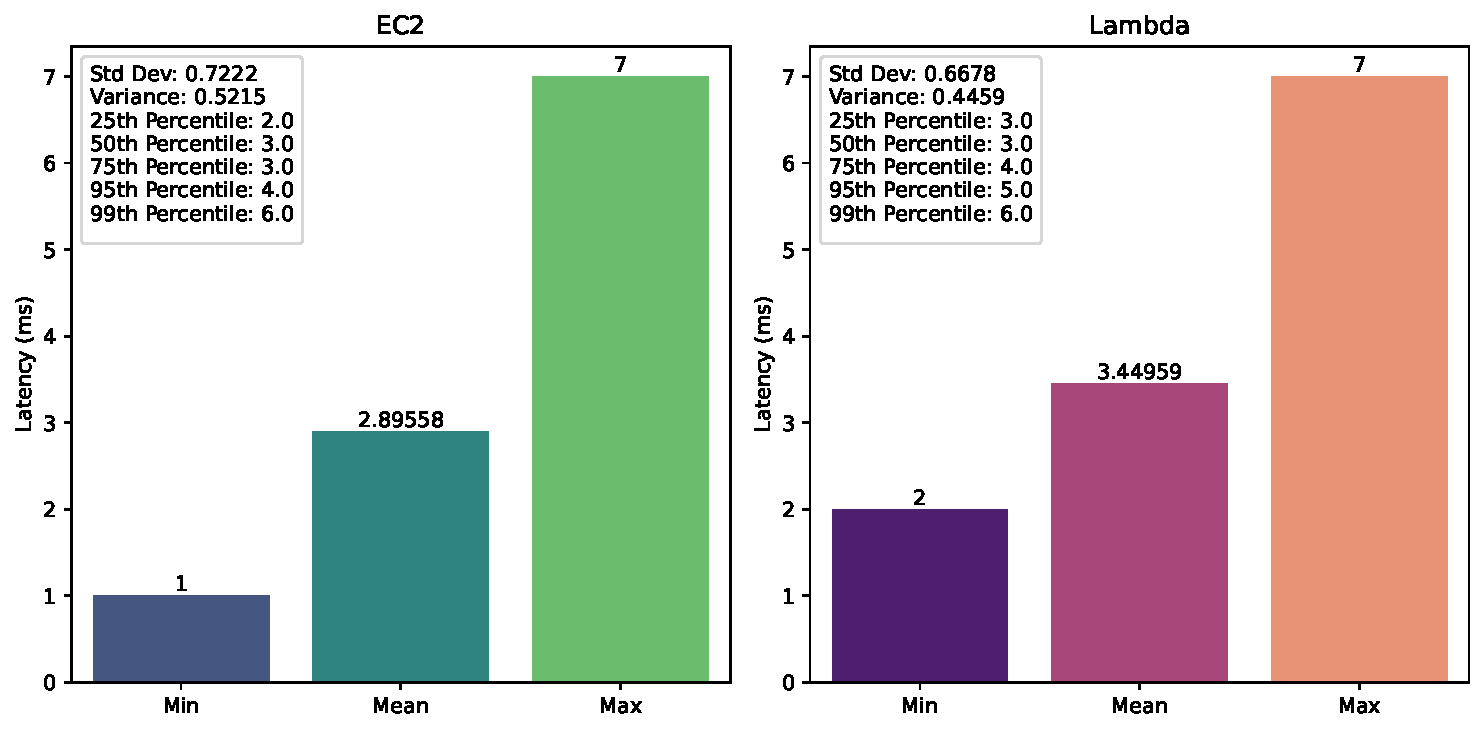
\includegraphics[width=\linewidth]{./fig/bar-dynamo-bursty.pdf}
		\caption{Burst Workload on DynamoDB}
		\label{fig:bar_ddb_bursty}
	\end{subfigure}
	\vfill
	\begin{subfigure}{0.49\linewidth}
		\centering
		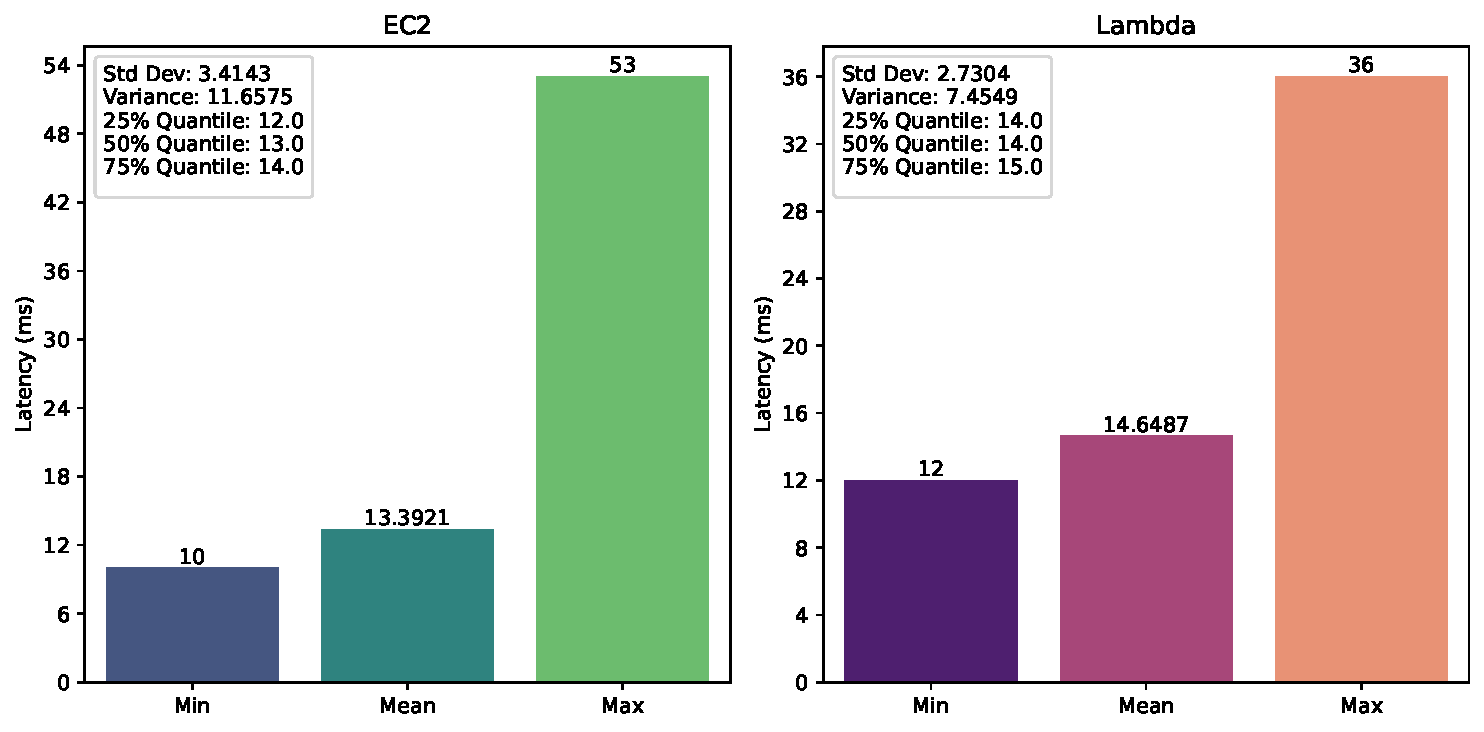
\includegraphics[width=\linewidth]{./fig/bar-s3-constant.pdf}
		\caption{Constant Workload on S3}
		\label{fig:bar_s3_const}
	\end{subfigure}
	\hfill
	\begin{subfigure}{0.49\linewidth}
		\centering
		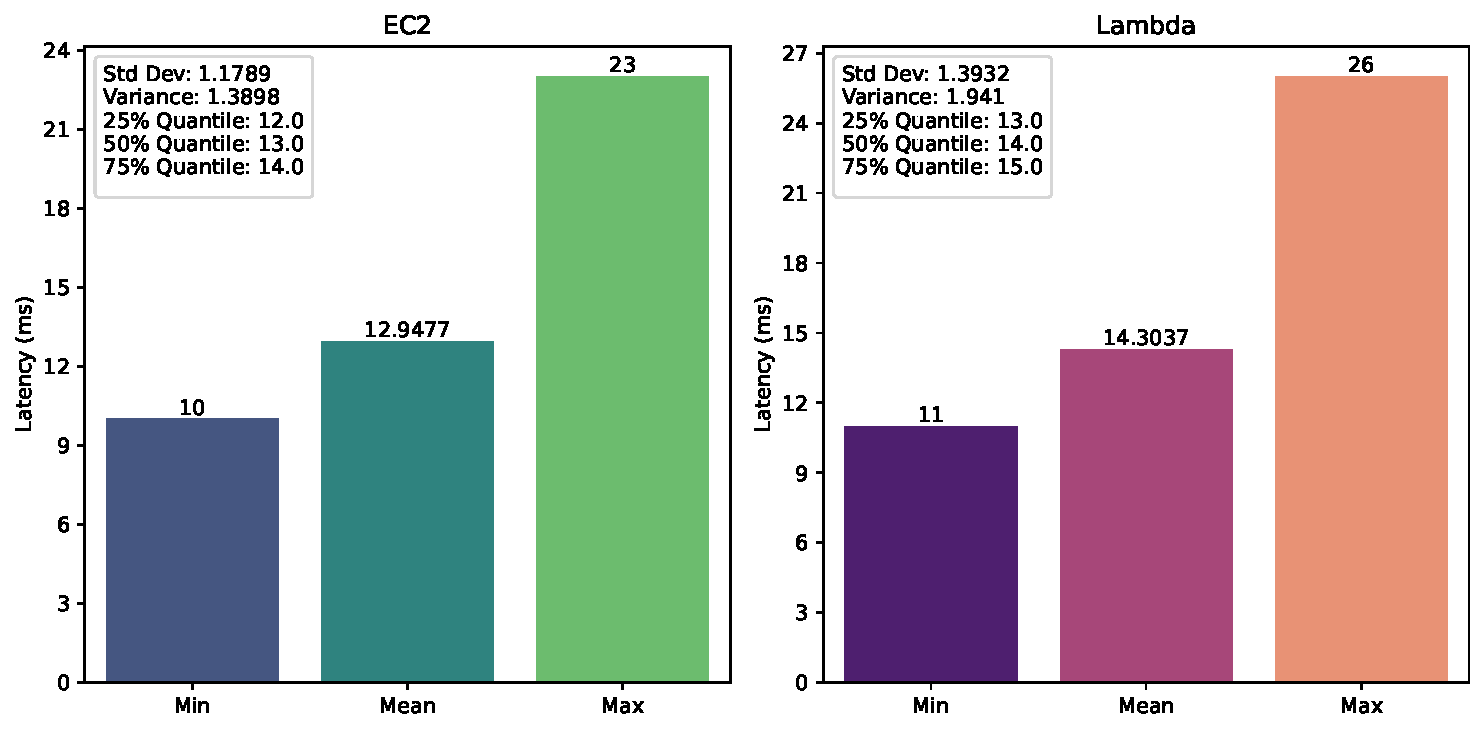
\includegraphics[width=\linewidth]{./fig/bar-s3-bursty.pdf}
		\caption{Burst Workload on S3}
		\label{fig:bar_s3_bursty}
	\end{subfigure}
	\caption{Aggregation of Latency Measurements}
	\label{fig:bar-plots}
\end{figure}

\begin{figure}[h]
	\begin{subfigure}{0.49\linewidth}
		\centering
		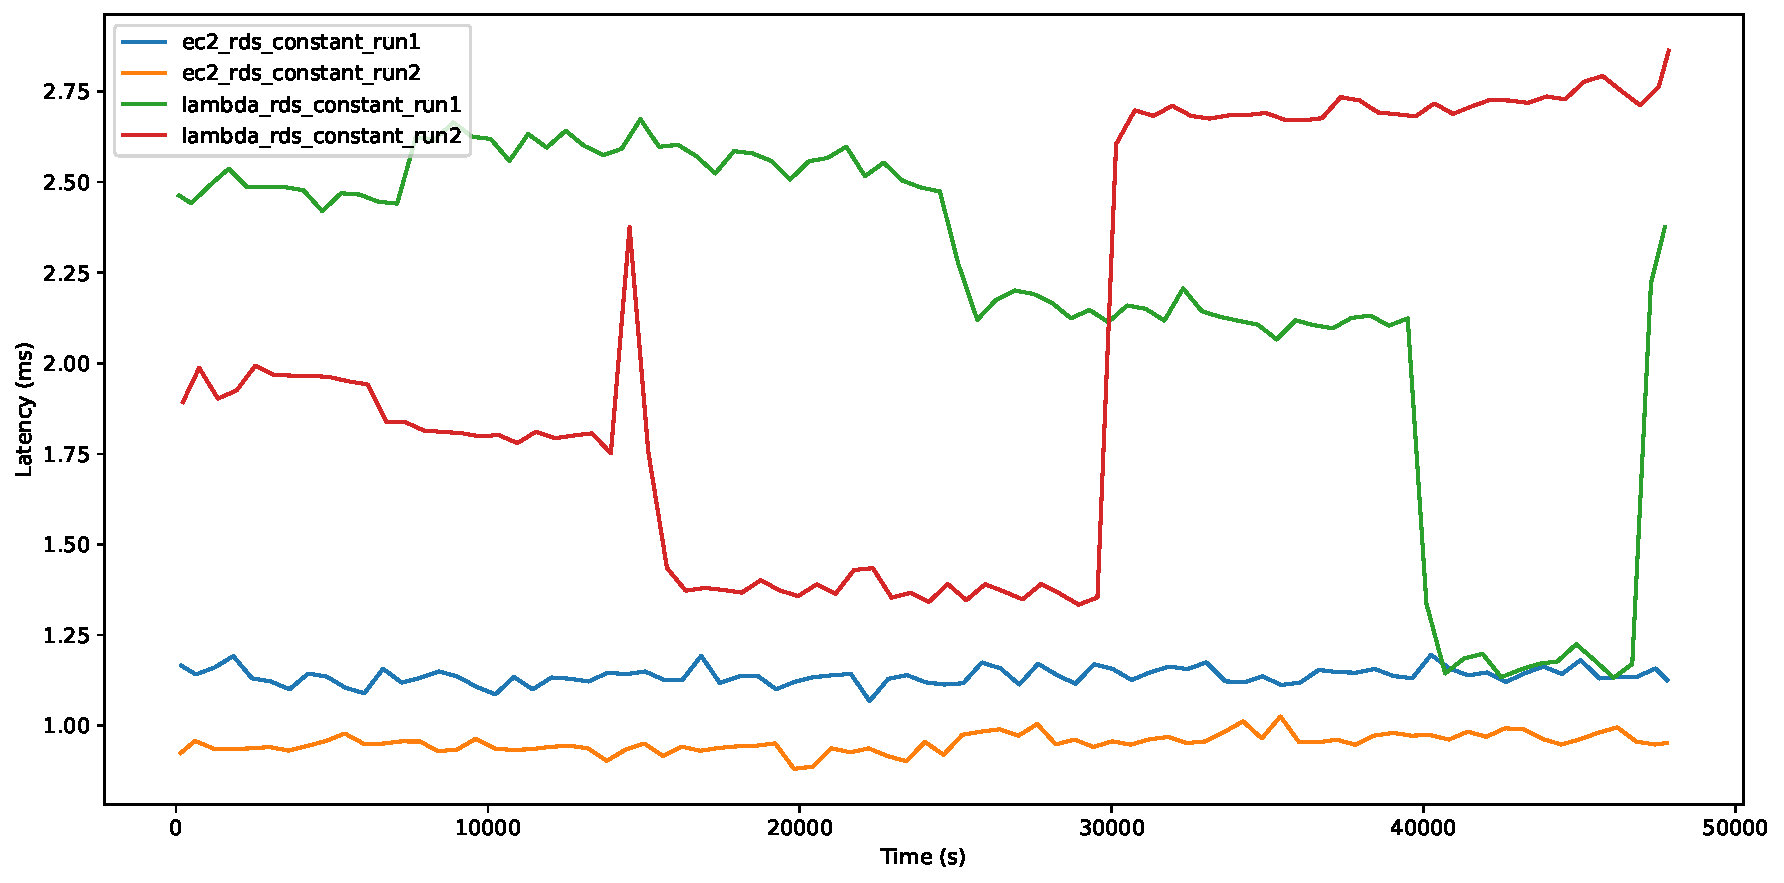
\includegraphics[width=\linewidth]{./fig/ts-rds-constant.pdf}
		\caption{Constant Workload on RDS}
		\label{fig:ts_rds_const}
	\end{subfigure}
	\hfill
	\begin{subfigure}{0.49\linewidth}
		\centering
		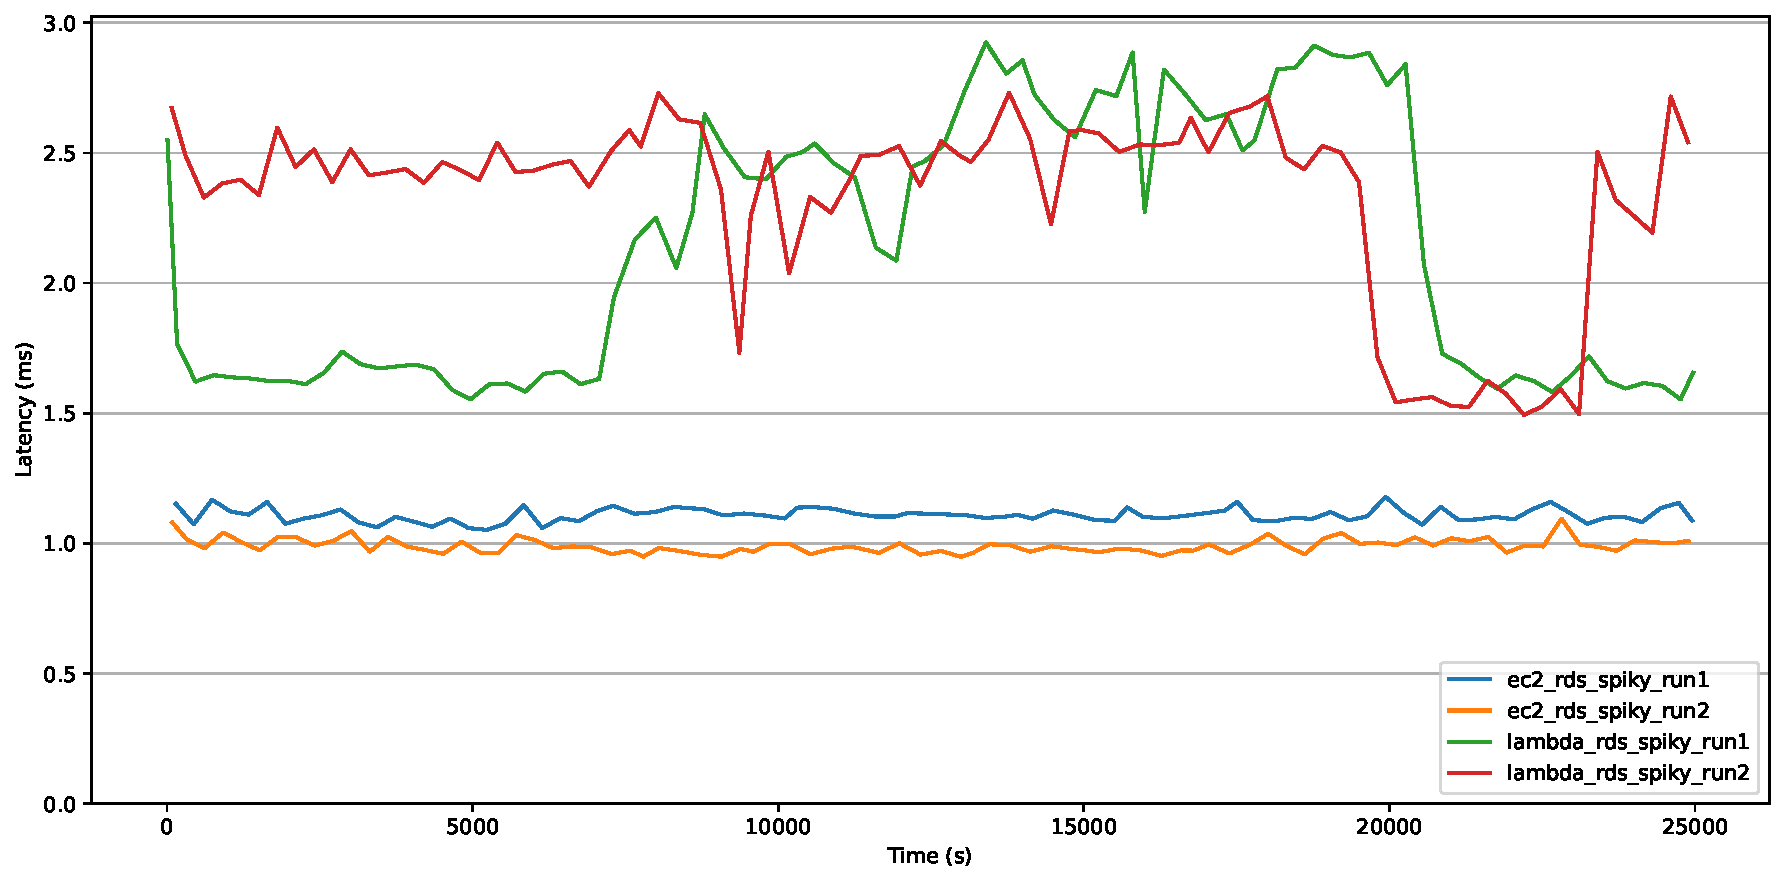
\includegraphics[width=\linewidth]{./fig/ts-rds-bursty.pdf}
		\caption{Burst Workload on RDS}
		\label{fig:ts_rds_bursty}
	\end{subfigure}
	\vfill
	\begin{subfigure}{0.49\linewidth}
		\centering
		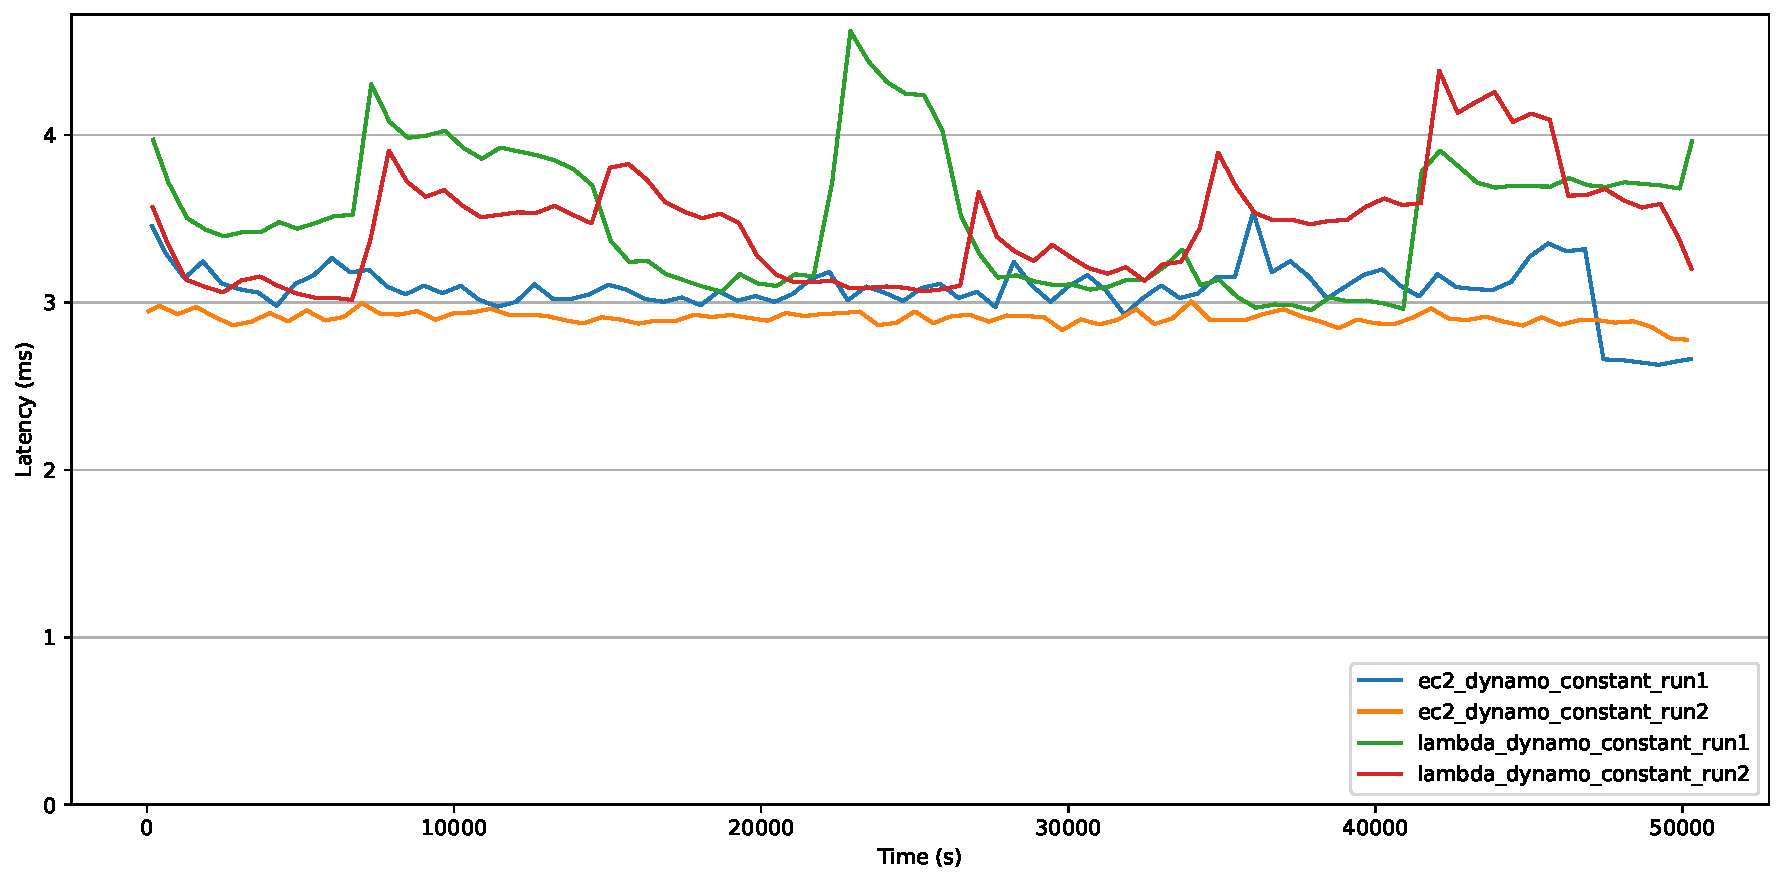
\includegraphics[width=\linewidth]{./fig/ts-dynamo-constant.pdf}
		\caption{Constant Workload on DynamoDB}
		\label{fig:ts_ddb_const}
	\end{subfigure}
	\hfill
	\begin{subfigure}{0.49\linewidth}
		\centering
		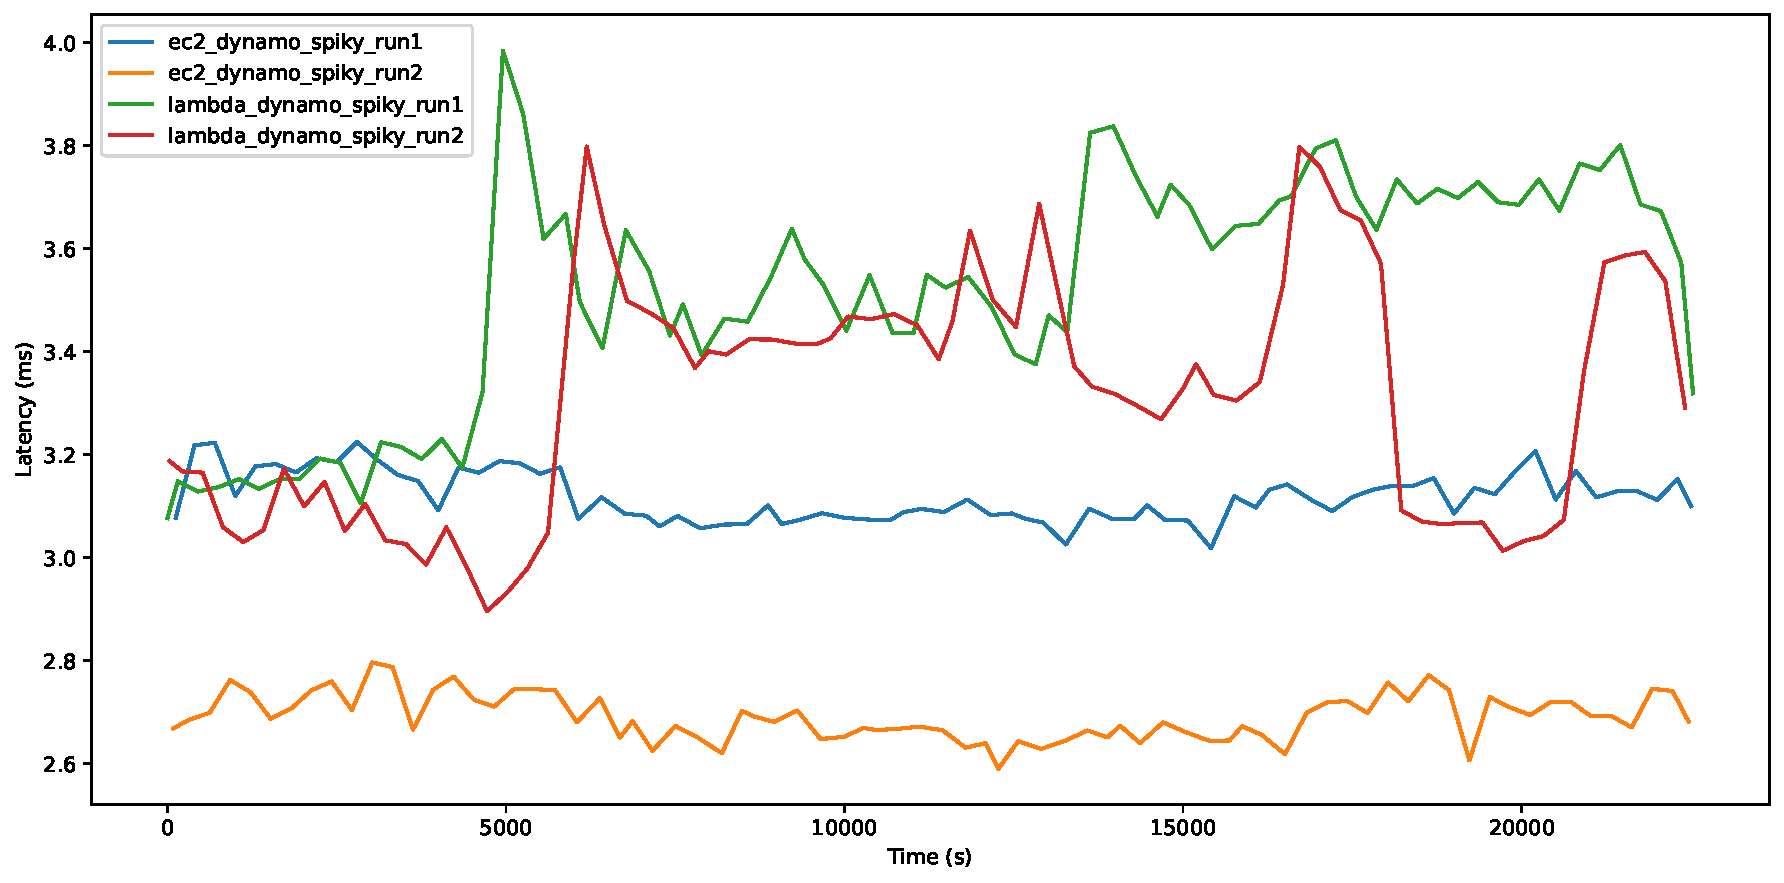
\includegraphics[width=\linewidth]{./fig/ts-dynamo-bursty.pdf}
		\caption{Burst Workload on DynamoDB}
		\label{fig:ts_ddb_bursty}
	\end{subfigure}
	\vfill
	\begin{subfigure}{0.49\linewidth}
		\centering
		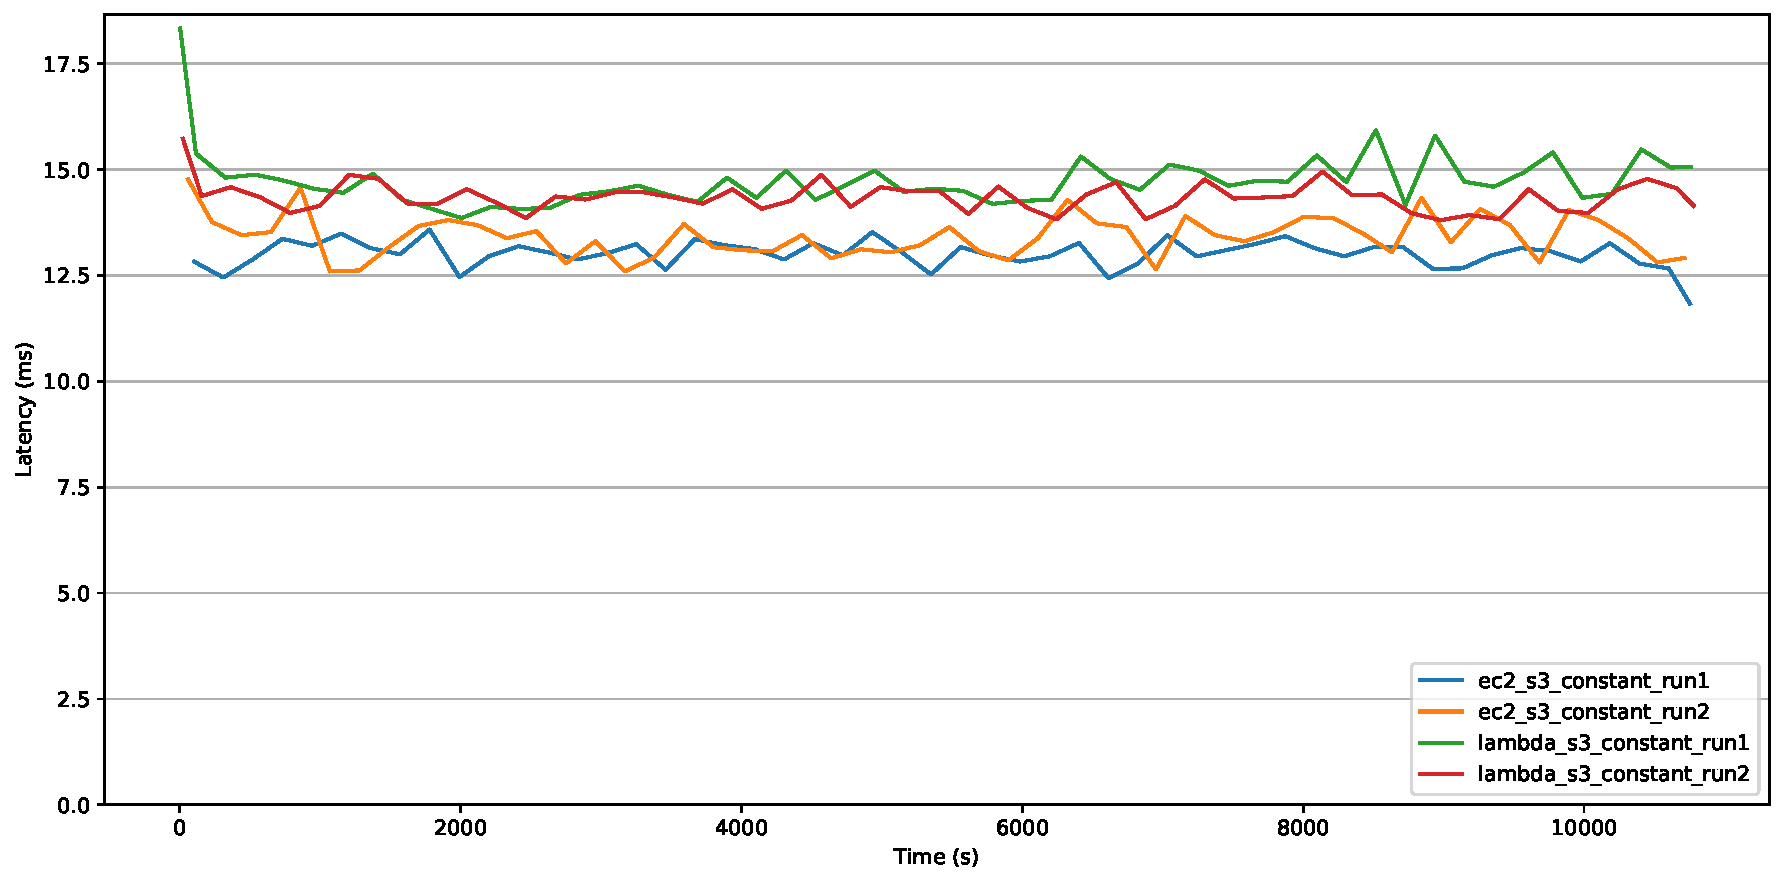
\includegraphics[width=\linewidth]{./fig/ts-s3-constant.pdf}
		\caption{Constant Workload on S3}
		\label{fig:ts_s3_const}
	\end{subfigure}
	\hfill
	\begin{subfigure}{0.49\linewidth}
		\centering
		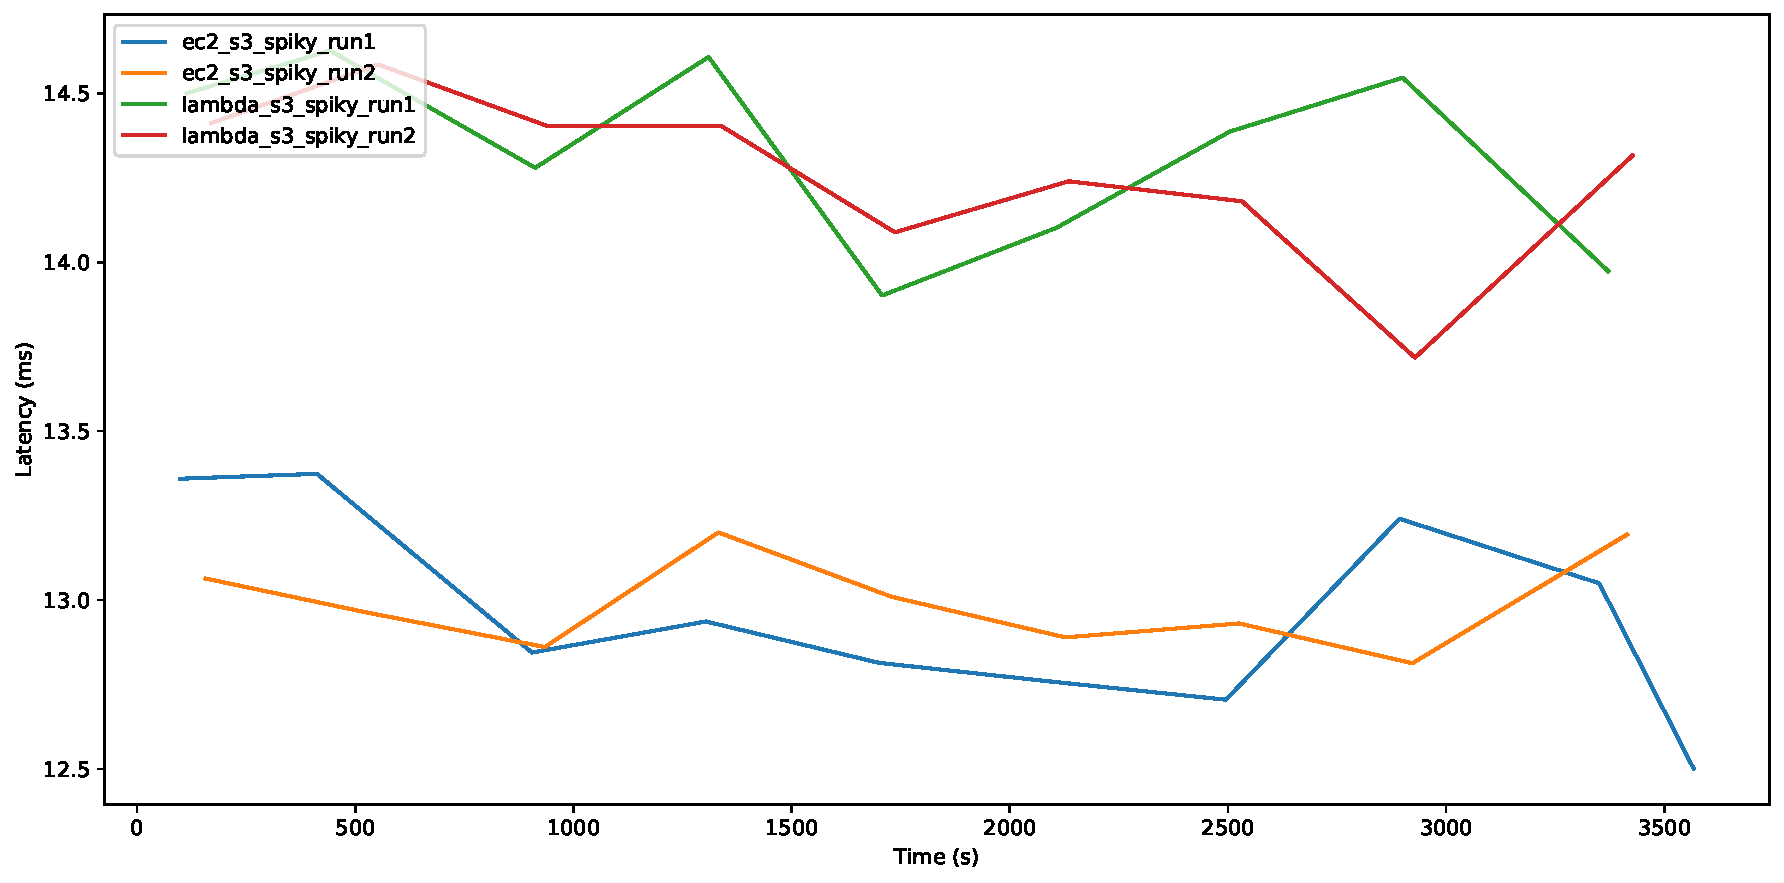
\includegraphics[width=\linewidth]{./fig/ts-s3-bursty.pdf}
		\caption{Burst Workload on S3}
		\label{fig:ts_s3_bursty}
	\end{subfigure}
	\caption{Time-Series Representation of Latency Measurements}
	\label{fig:ts-plots}
\end{figure}

